\chapter{Introduction}
\label{sec:introduction}

this is the introduction. Lorem ipsum dolor sit amet, consectetur adipisicing elit, sed do eiusmod
tempor incididunt ut labore et dolore magna aliqua. Ut enim ad minim veniam,
quis nostrud exercitation ullamco laboris nisi ut aliquip ex ea commodo
consequat. Duis aute irure dolor in reprehenderit in voluptate velit esse
cillum dolore eu fugiat nulla pariatur. 

\section{anImage}
\label{anImage}
Also, the analysis itself is kept modular, so the spectral processing, the peak finding or the audio input can easily be exchanged.
The whole structure of the Max patch follows the structure given in fig. ~\ref{fig:problem}. An overview of the complete Patch is given in fig. ~\ref{fig:maxOverview}.

\begin{figure}[H]
	\begin{center}
		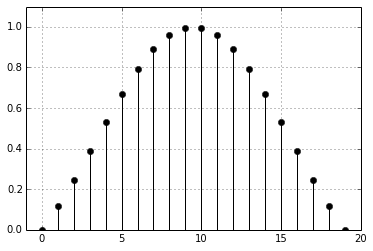
\includegraphics[width = 14cm]{img/BAK4_final_12_0.png}
		\caption{A great description}
		\label{fig:maxOverview}
	\end{center}
\end{figure}


\section{quotation}
\label{quotation}
A reference to the bibliography and a footnote link. \citep[see][p. 230]{cook_real_2002}. A good example of such a decomposition is the Kelly Lochbaum vocal tract model as described by \citep{smith_physical_2010}\footnote{\texttt{https://ccrma.stanford.edu/\~{}jos/pasp/Ideal\_Acoustic\_Tube.html}}.


\section{Math}
\label{Math}
A test of in line math \(\phi^2sin(\pi)\) test
Some line tests
some more
some extra equation 
\begin{align}
	2*sin \pi
\end{align}


\section{Code}
\label{Code}
Go for Google to get syntax highlighting. It is possible. If python/Julia/R code is used, look at ipython notebook (export to latex)
\begin{verbatim}
while True:
	print ('Hello world')
\end{verbatim}


\section{Blockdiagrams}
\label{Blockdiagrams}

\begin{figure}[htb]
  \centering  
  
  \label{fig:problem}
	\begin{tikzpicture}[auto, thick, node distance=2.1cm, >=triangle 45]
	
		\draw node at (0,0) [block] (ir) {\Large$Impulse\ Resonse$};
		\draw node [block, below of=ir] (FFT) {\Large$Extraction\ of\ Resonance\ Signal\ Spectrum$};
		\draw node [block, below of=FFT] (choose) {\Large$Finding\ the\ Most\ important\ Frequencies$};
		\draw node [block, below of=choose] (pars) {\Large$Determining\ amplitude\ and\ decay$};
		
		
		\draw[->] (ir) -- node {}(FFT);
		\draw[->] (FFT) -- node {}(choose);
		\draw[->] (choose) -- node {}(pars);
		
	\end{tikzpicture}
\caption{sub-problems of parameter extraction}
\end{figure}

The problem of obtaining a proper impulse response is not discussed here, rather the emphasis lies on the automated or semi-automated processing of the data. Each of the blocks in figure ~\ref{fig:problem} is a complex process of its own. Therefore each of these will be treated individually here. \\


tempor incididunt ut labore et dolore magna aliqua. Ut enim ad minim veniam,
quis nostrud exercitation ullamco laboris nisi ut aliquip ex ea commodo
consequat. Duis aute irure dolor in reprehenderit in voluptate velit esse
cillum dolore eu fugiat nulla pariatur. Excepteur sint occaecat cupidatat non
proident, sunt in culpa qui officia deserunt mollit anim id est laborum.Lorem ipsum dolor sit amet, consectetur adipisicing elit, sed do eiusmod
tempor incididunt ut labore et dolore magna aliqua. Ut enim ad minim veniam,
quis nostrud exercitation ullamco laboris nisi ut aliquip ex ea commodo
consequat. Duis aute irure dolor in reprehenderit in voluptate velit esse
cillum dolore eu fugiat nulla pariatur. Excepteur sint occaecat cupidatat non
proident, sunt in culpa qui officia deserunt mollit anim id est laborum.Lorem ipsum dolor sit amet, consectetur adipisicing elit, sed do eiusmod
tempor incididunt ut labore et dolore magna aliqua. Ut enim ad minim veniam,
quis nostrud exercitation ullamco laboris nisi ut aliquip ex ea commodo
consequat. Duis aute irure dolor in reprehenderit in voluptate velit esse
cillum dolore eu fugiat nulla pariatur. Excepteur sint occaecat cupidatat non
proident, sunt in culpa qui officia deserunt mollit anim id est laborum.